\problemname{Gwen's Gift}

Gwen loves most numbers. In fact, she loves every number that is \textit{not} a multiple of $n$ (she really hates the number $n$).
For her friends' birthdays this year, Gwen has decided to draw each of them a sequence of $n-1$ flowers.
Each of the flowers will contain between $1$ and $n-1$ flower petals (inclusive).
Because of her hatred of multiples of $n$, the total number of petals in
any non-empty contiguous subsequence of flowers cannot be a multiple of $n$. For example, if $n = 5$, then the top two paintings are valid,
while the bottom painting is not valid since the second, third and fourth flowers have a total of $10$ petals.
(The top two images are Sample Input $3$ and $4$.)

\begin{center}
 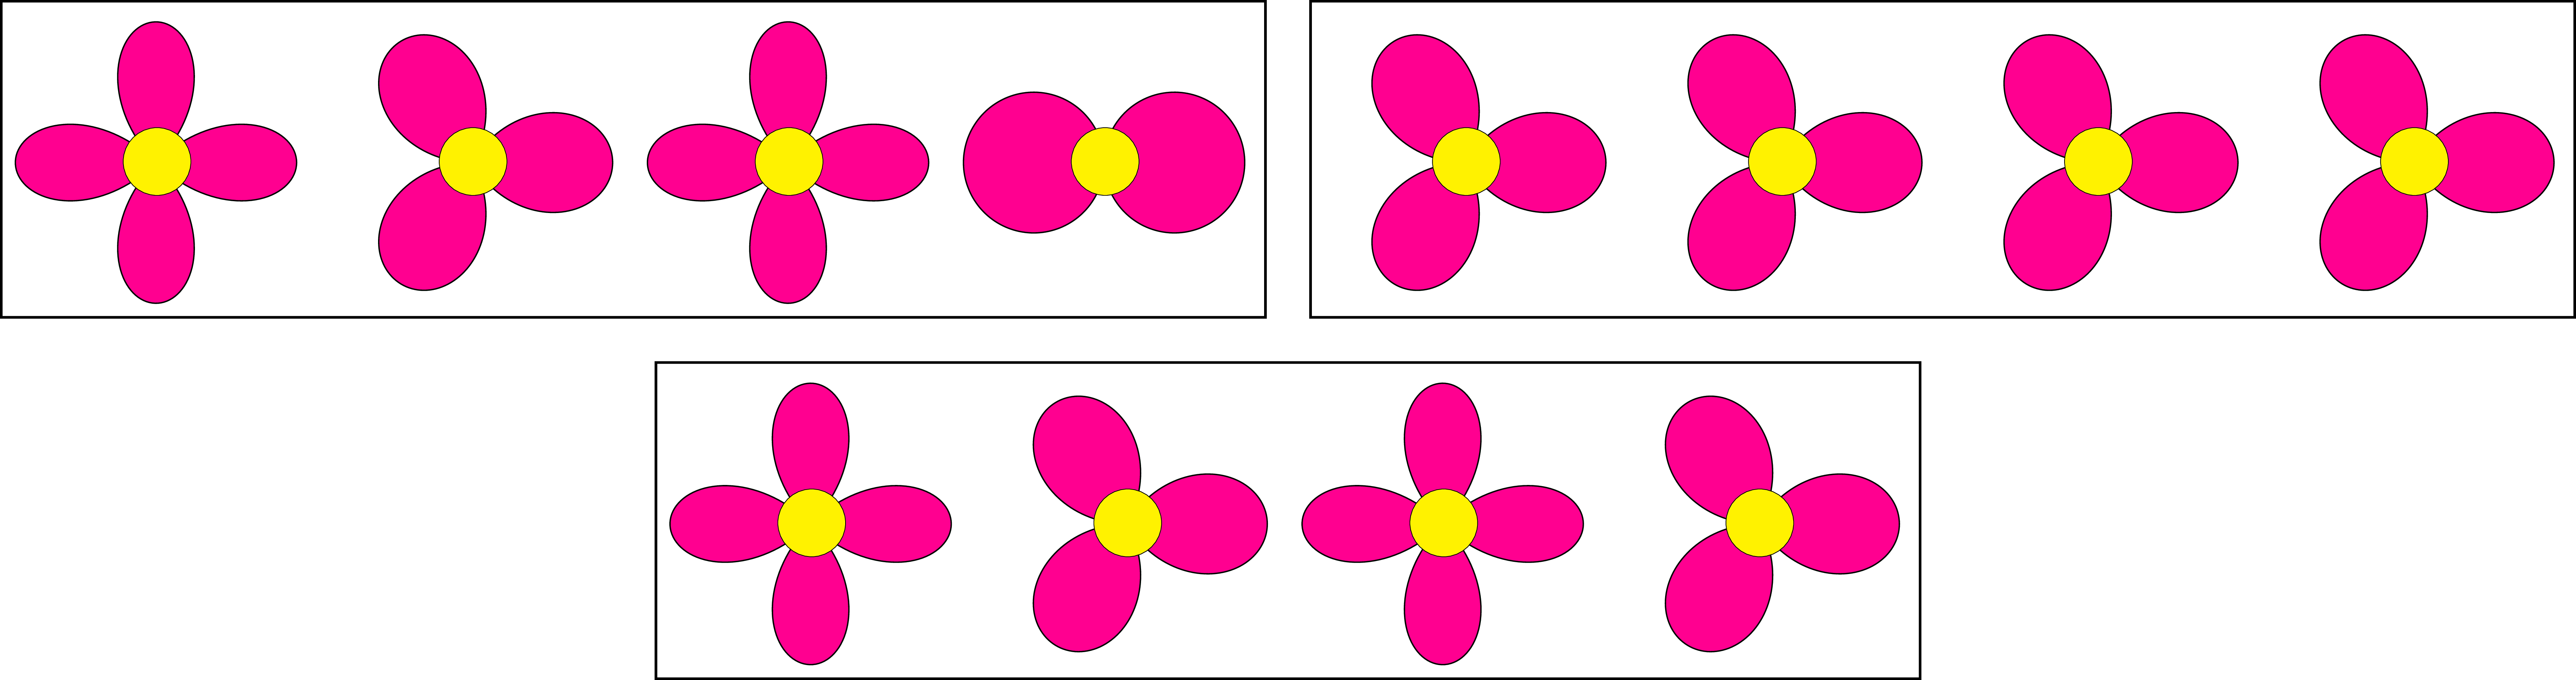
\includegraphics[width=0.9\textwidth]{gift-flowers.png}
\end{center}

Gwen wants her paintings to be unique, so no two paintings will have
the same sequence of flowers.  To keep track of this, Gwen recorded
each painting as a sequence of $n-1$ numbers specifying the number of
petals in each flower from left to right.  She has written down all
valid sequences of length $n-1$ in lexicographical order. A sequence
$a_1,a_2,\dots, a_{n-1}$ is lexicographically smaller than 
$b_1, b_2, \dots, b_{n-1}$ if there exists an index $k$ such that $a_i = b_i$
for $i < k$ and $a_k < b_k$.

What is the $k$th sequence on Gwen's list?


\section*{Input}

The input consists of a single line containing two integers $n$~($2 \leq n \leq 1\,000$),
which is Gwen's hated number, and $k$~($1 \leq k \leq 10^{18}$), which is the index of the valid sequence in question
if all valid sequences were ordered lexicographically.
It is guaranteed that there exist at least $k$ valid sequences for this value of $n$.


\section*{Output}

Display the $k$th sequence on Gwen's list.

